\section{Introduction}
Objects with high-resolution, heterogeneous material properties are everywhere:
from the output of multimaterial 3D printers 
to virtual characters gracing the screen in summer blockbusters.
Designing such objects is made possible by the tight coupling of design
tools and numerical simulation which allows designers 
(or optimization algorithms) to update geometry or material parameters 
and subsequently estimate the physical effects of the change.
Fast, accurate simulation techniques that can handle runtime changes 
in geometry and material composition are a necessity for such iterative design algorithms.
The gold standard technique for estimating the mechanical behavior
of a deformable object under load is the finite element method (FEM).
While accurate, FEM is notoriously slow,
making it a major bottleneck in the iterative design process.
For this reason, there have been a large number of works on speeding up FEM simulations,
and these speed improvements have enabled FEM to be used in many performance critical tasks
such as computer animation, surgical training, and virtual/augmented reality.
Unfortunately, even though techniques such as model reduction or numerical coarsening 
can achieve order-of-magnitude performance increases,
they require expensive precomputation phases, typically on the order of minutes
for large meshes. This precomputation requires knowledge of an object’s 
geometry and material composition a priori,
something that is not known during a design task.
When the user updates the model by changing the geometry or the material distribution,
the preprocessing step must be run again.
Since this step is inside the design loop,
the user cannot get rapid feedback on the changes made to the object.
Additionally, many existing methods assume the object only undergoes small deformations
with known boundary conditions.
Extensions of these methods to large deformations with varying boundary conditions
severely increase the algorithm complexity and quickly diminishes the performance improvements.

We propose coarsening algorithms based on standard FEM
without introducing new types of spatial discretization which increases
algorithmic complexity.
Our algorithm reduces the element count by using coarser elements with data-driven
material properties suitable for design tasks.
The data is acquired before design iterations either from high-resolution simulations or from measurements.
At runtime, precomputed element material properties are applied to a coarse discretization.
The coarsened FEM models can accommodate varying geometry,
material assignments and boundary conditions of an elastic object.
We will fabricate exemplar objects and design physics experiments to validate that our coarsened approximations are sufficiently predictive of object behaviors.
An overview of the pipeline is shown in figure~\ref{fig:overview}.
\begin{figure}[ht]
	\centering
	\subcaptionbox{\label{fig:typical}Typical methods}{
		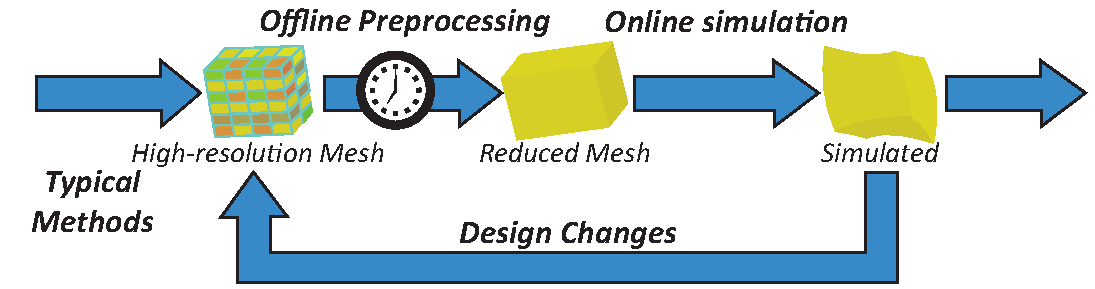
\includegraphics[width=0.7\columnwidth]{images/typical1.pdf}
	}
	\subcaptionbox{\label{fig:ours}Our method}{
		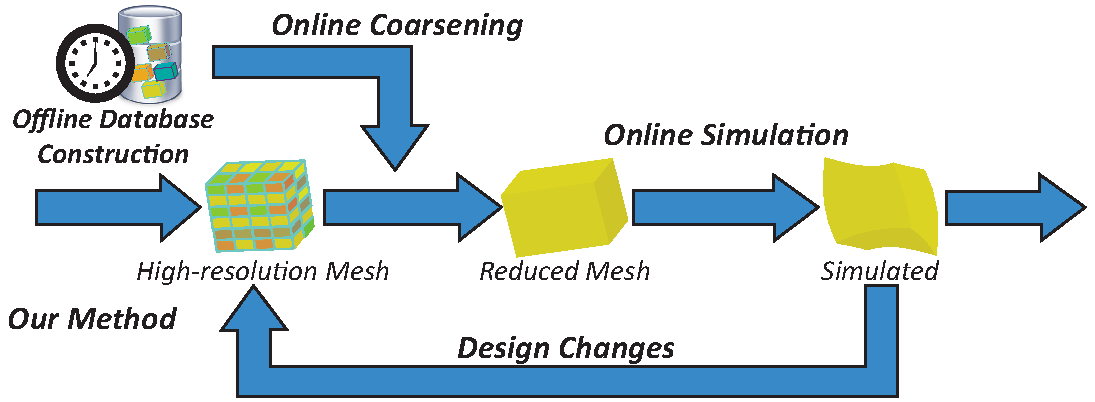
\includegraphics[width=0.7\columnwidth]{images/typical2.pdf}
	}
	\caption{
		(a) In a typical method, the preprocessing step of reducing element count is performed for every design change, making the design loop slow.
		(b) In our method, we move the time-consuming offline computation outside of the design loop.
	}
	\label{fig:overview}
\end{figure}
